\section{Implementation}
The data link layer is implemented as a \custtt{DataLinkLayer} class and a
\custtt{Frame} class as shown in \ref{fig:class_diag_for_datalink}. The
\custtt{DataLinkLayer} object is instantiated by the \custtt{BackBone} class and
controls the network token and the processing of frames into datagrams and vice
versa. When instantiated, the address and token are controlled by arguments. The
Frame objects and datagram objects are instantiated in buffers by the backbone
and presented to the data link layer as method arguments.

\begin{figure}[htb]
	\centering
	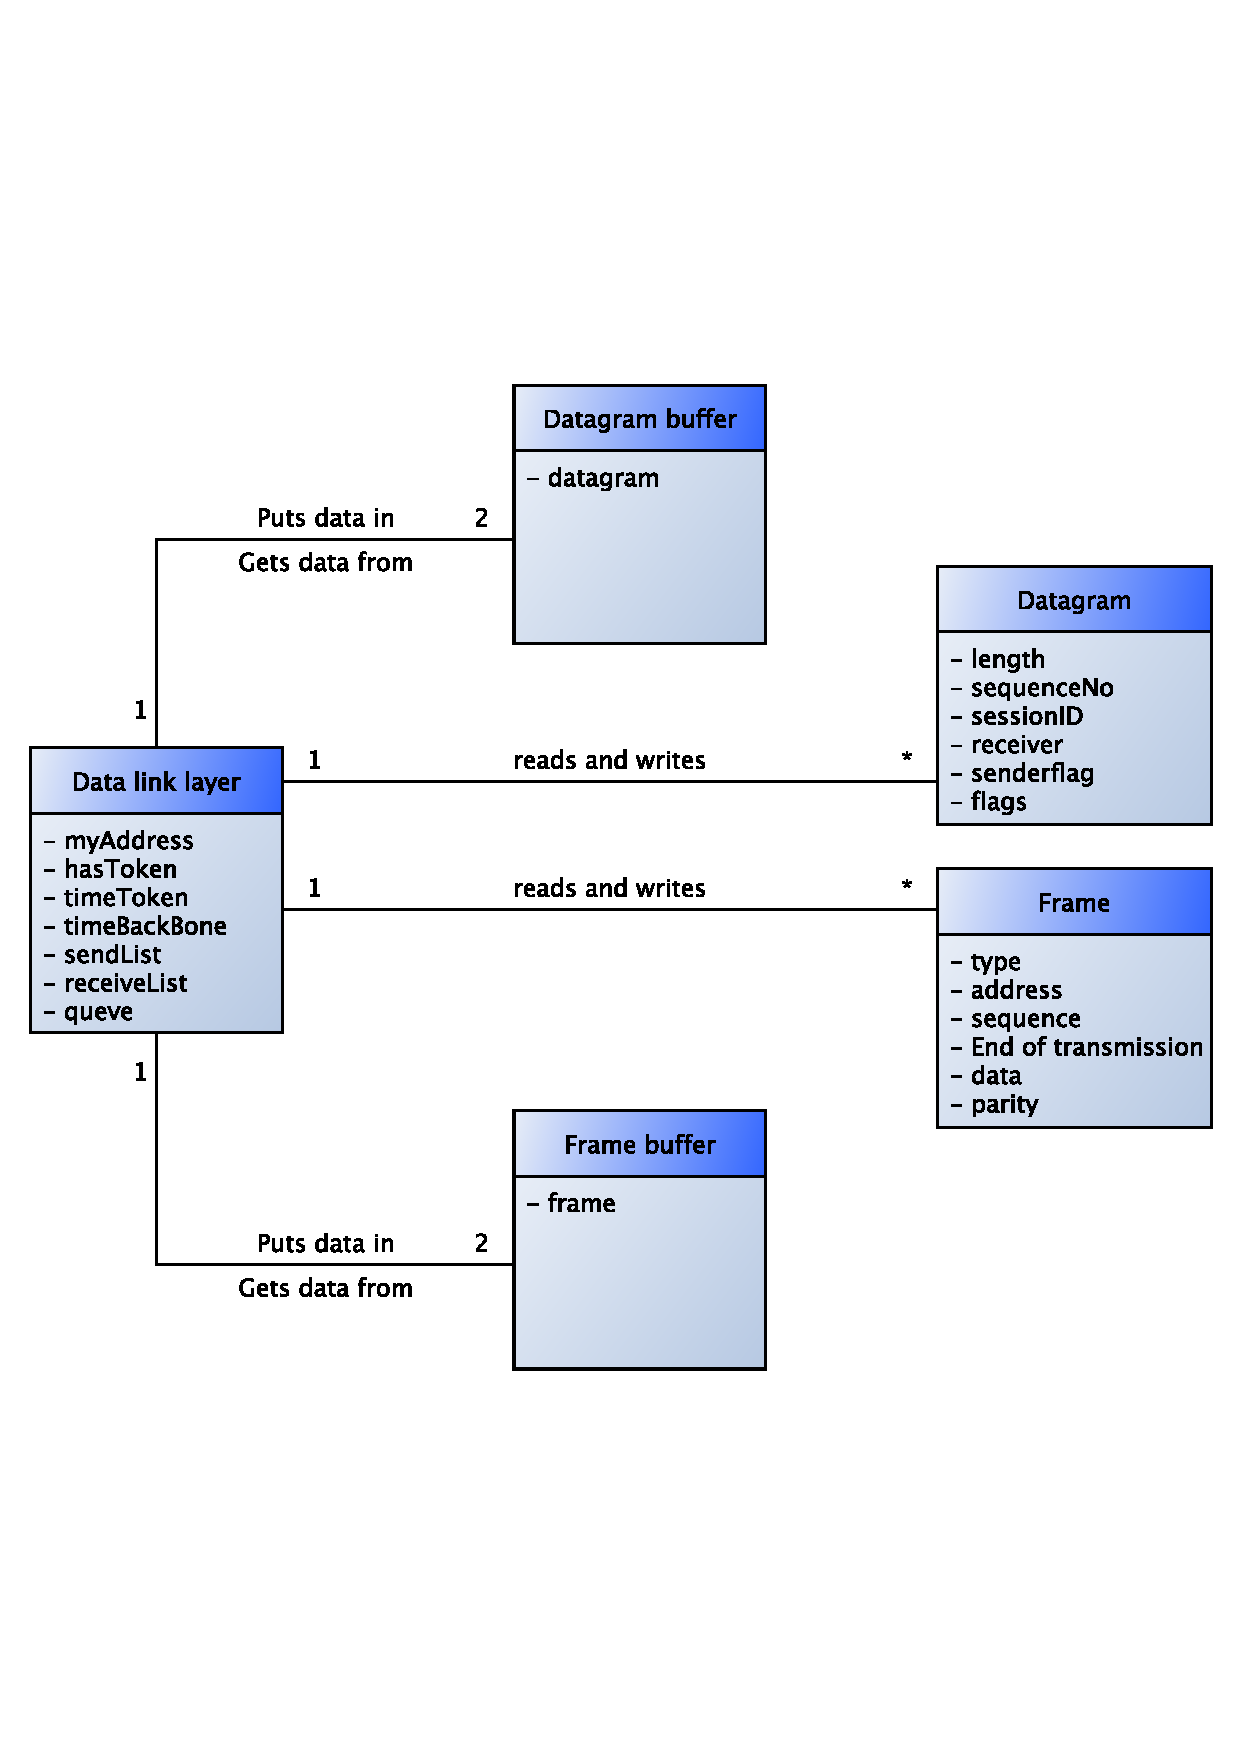
\includegraphics[scale=0.58,trim=0 170 0 170]{dll_domainmodel.pdf}
	\caption{Domain model for data link layer.}
	\label{fig:class_diag_for_datalink}	
\end{figure}

Two public methods are used to call the data link layer, one for upwards traffic
(\custtt{decode}) and one for downwards traffic (\custtt{encode}). Both methods are called with
pointers to the four accessible buffers as arguments. Furthermore the backbone
can call a method (\custtt{needs\-Attention}) to know whether the data link layer needs
extraordinary attention because a timer has run out. Another method
(\custtt{canTransmit}) tells the backbone whether the data link layer object holds the
network token and thereby is able to send encoded data.

\begin{figure}[htb]
	\centering
	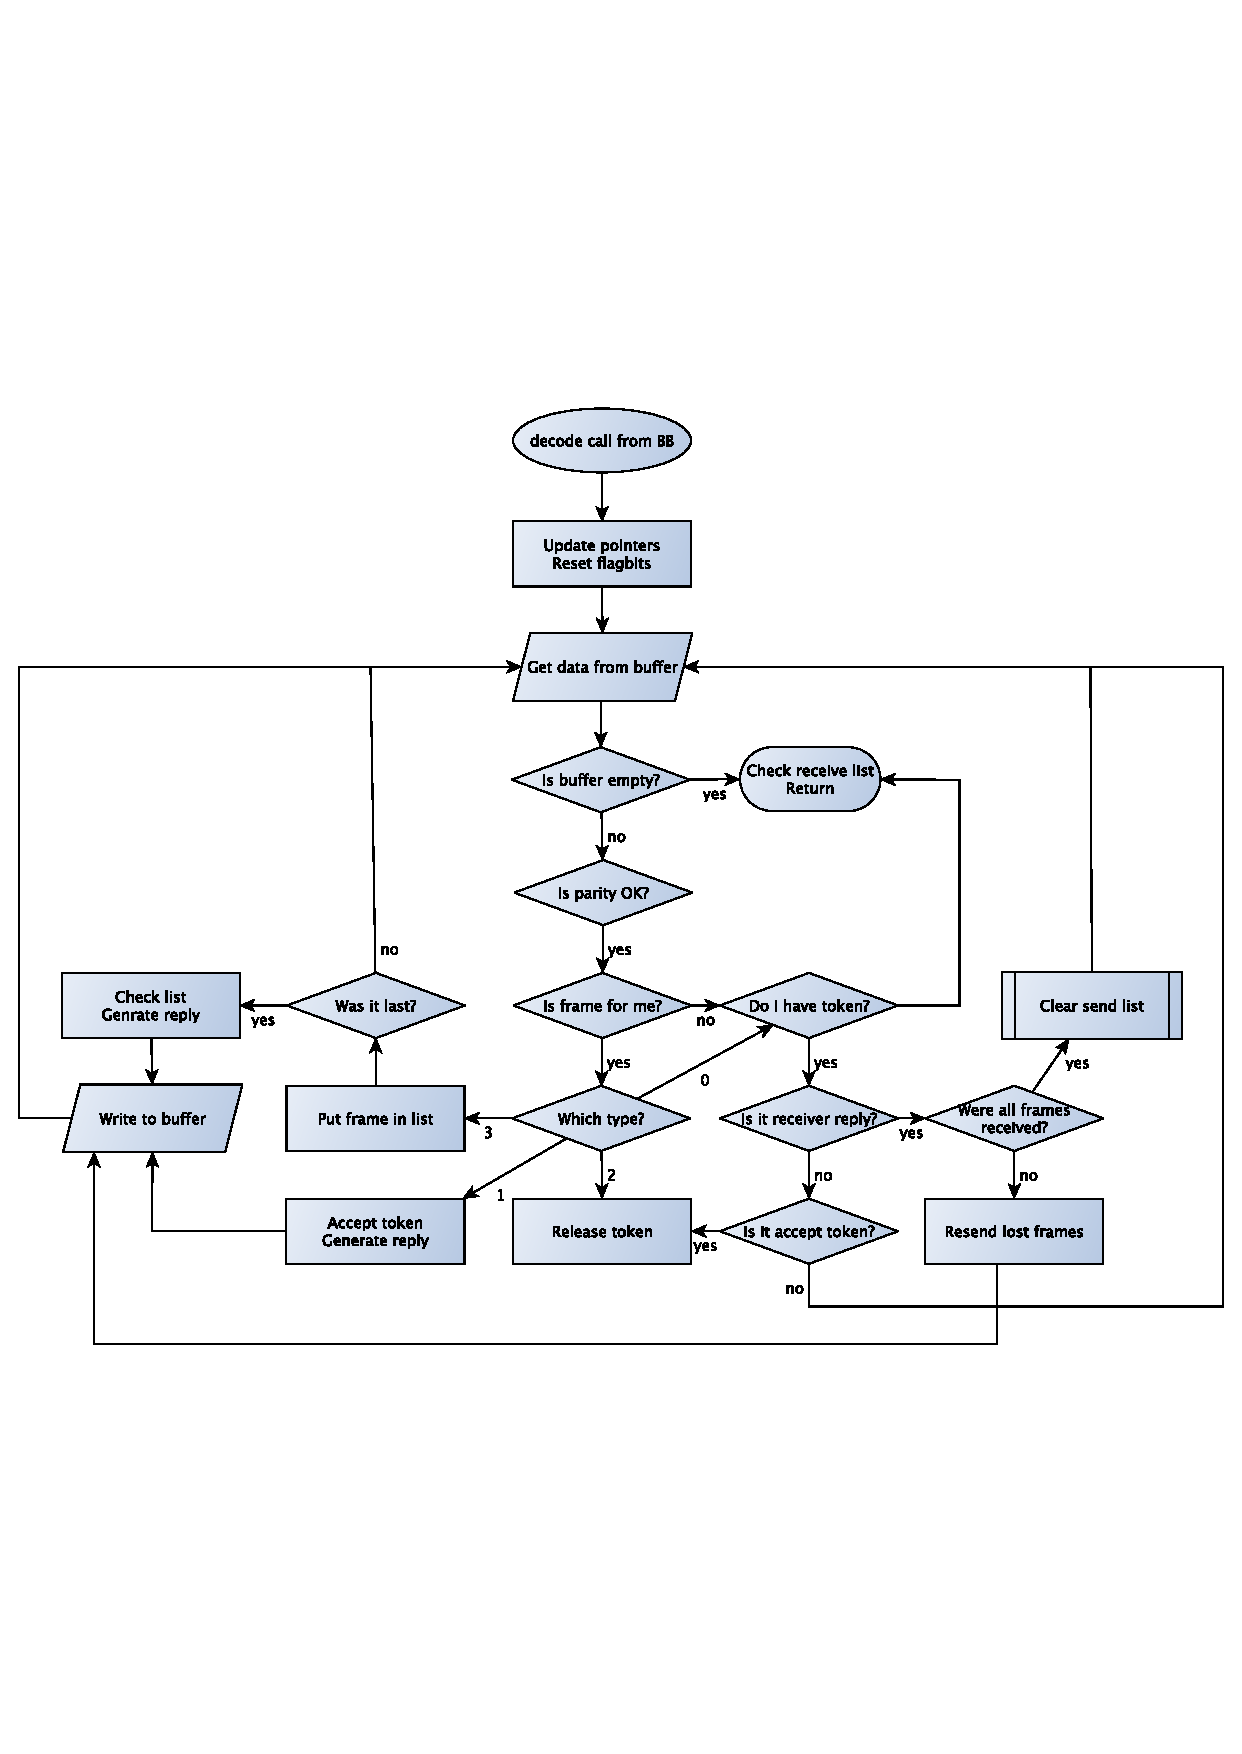
\includegraphics[scale=0.58,trim=0 190 0 190]{dll_flow_decode.pdf}
	\caption{Flow chart for data link layer decode method.}
	\label{fig:dll_flow_decode}	
\end{figure}

The methods of the classes are developed to realize the
flowcharts shown in Figure \ref{fig:dll_flow_encode} and
\ref{fig:dll_flow_decode} of the data link layer. Decisions on whether to implement a method in one class or another is done using the expert pattern.

\begin{figure}[htb]
	\begin{center}
	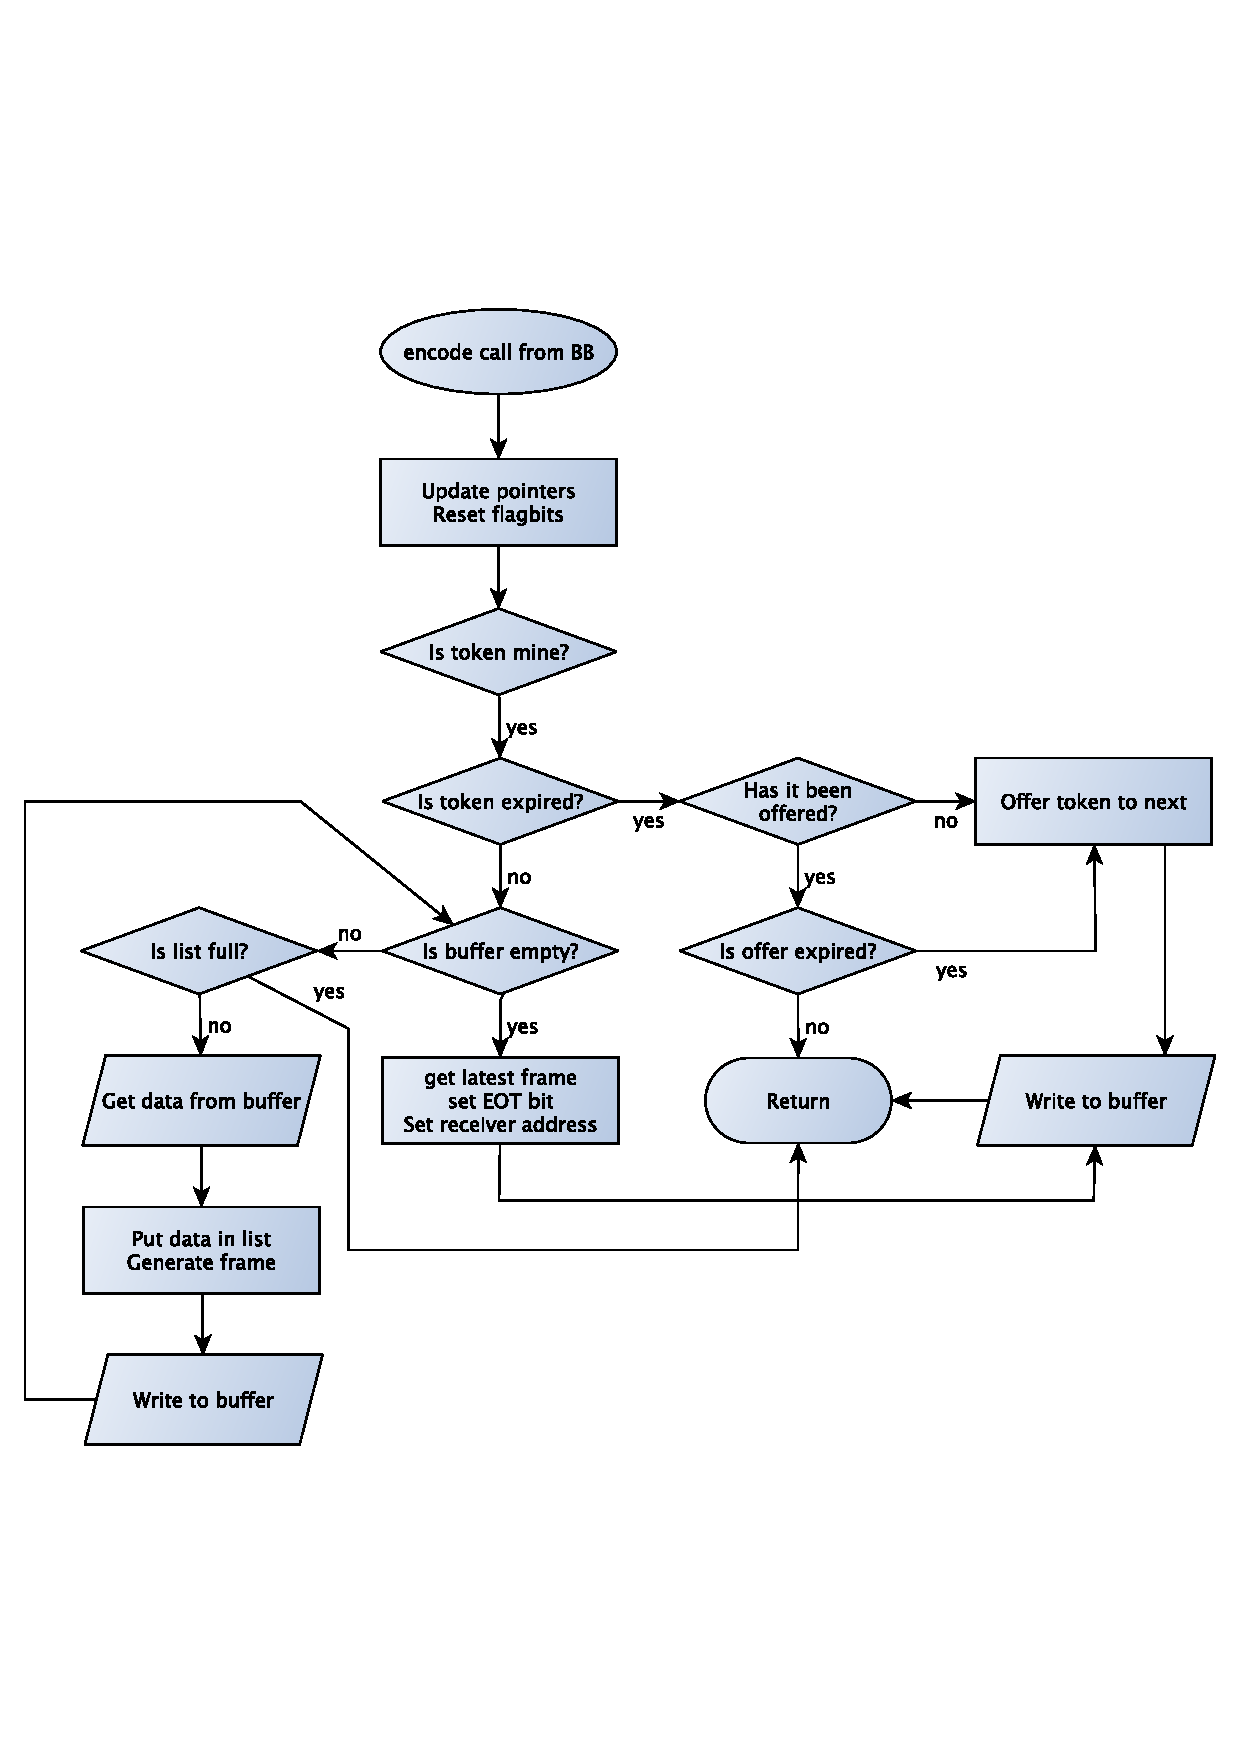
\includegraphics[scale=0.58,trim=0 140 0 140]{dll_flow_encode.pdf}
	\caption{Flow chart for data link layer encode method.}
	\label{fig:dll_flow_encode}	
	\end{center}
\end{figure}

The token network is implemented to deal with the cases shown in Figure
\ref{fig:dll_token_network}. It is important that the network is implemented to
support the half duplex nature of the DTMF tone based network, since any
collision would lead to errors. This is implemented by the EOT bit, that has to
be received before a non token holder can talk. The token holder waits a specified
amount of time after sending the EOT-bit before re-transmitting or moving on.

\begin{figure}[htb]
	\begin{center}
	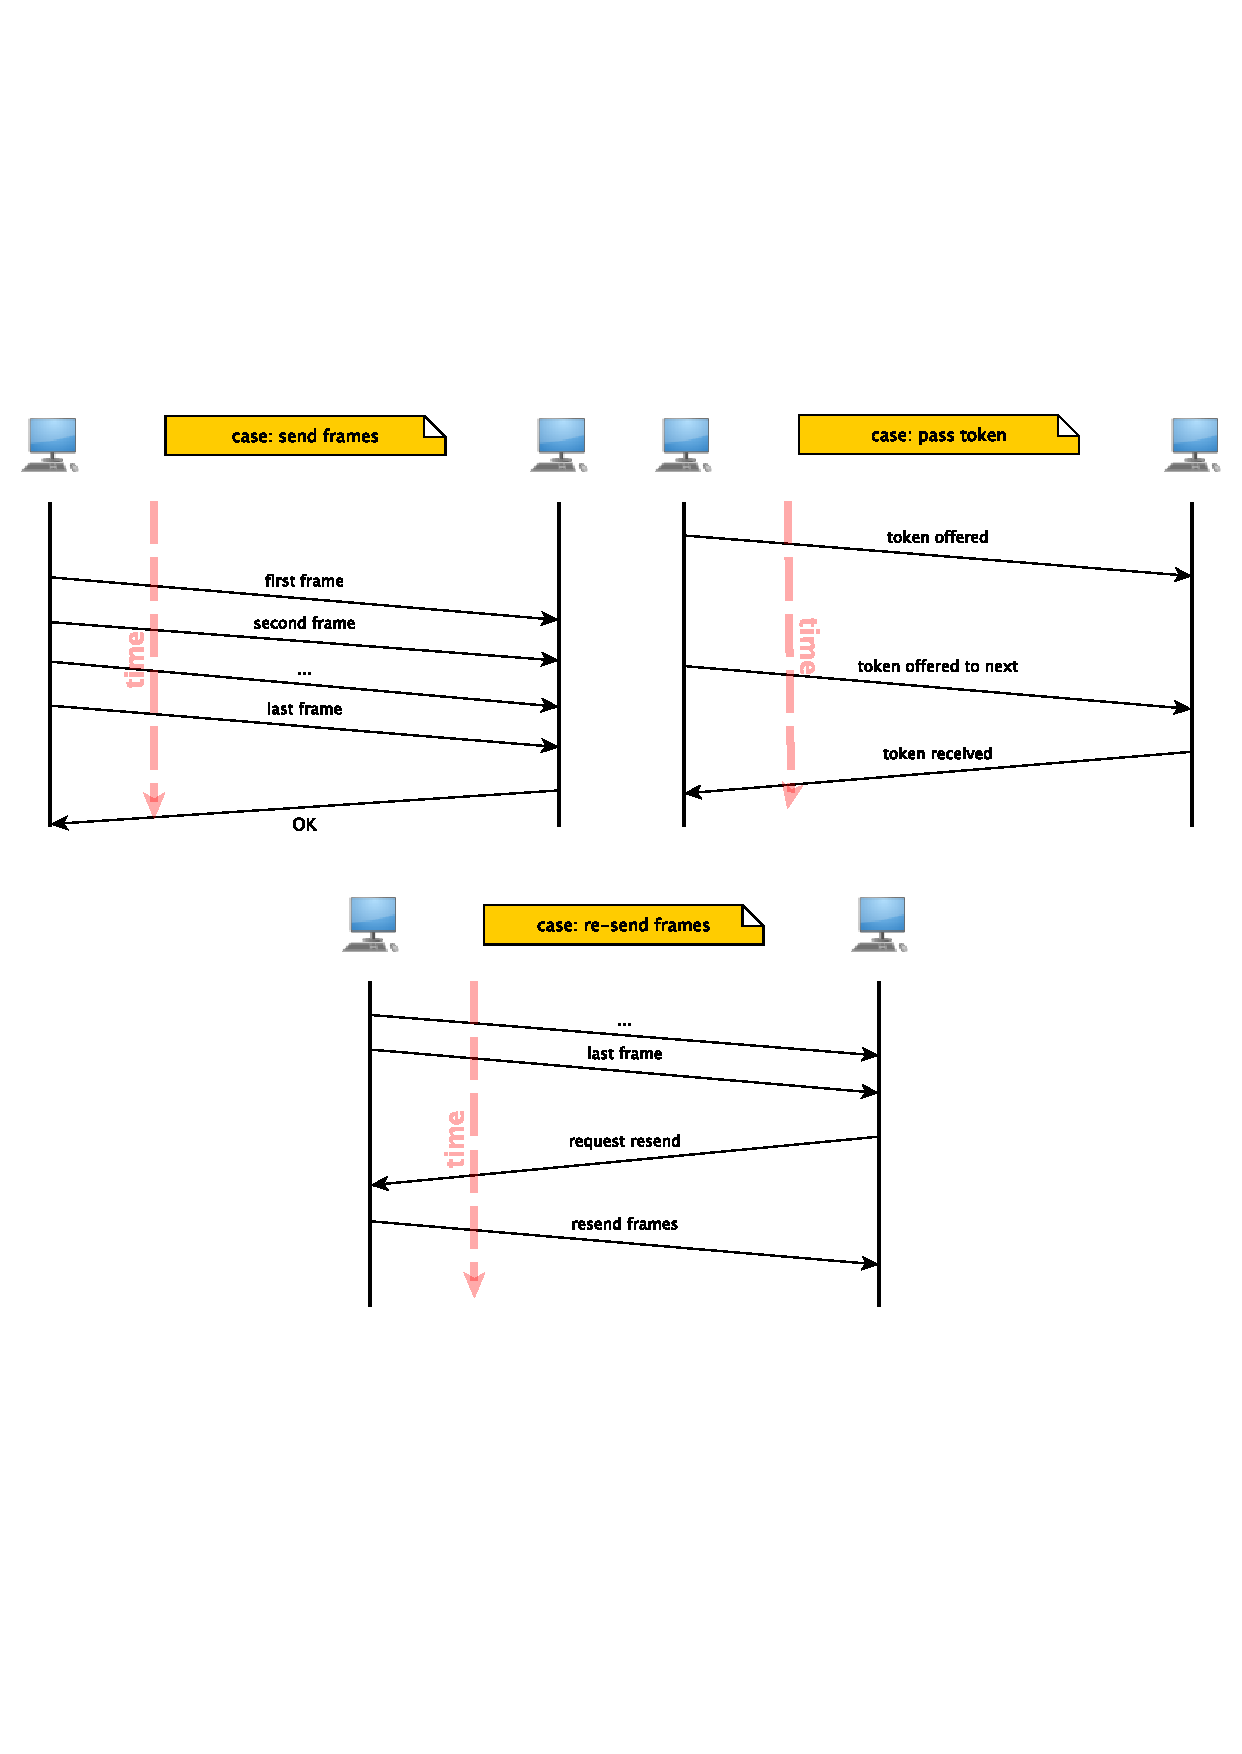
\includegraphics[scale=0.58,trim=0 200 0 200]{dll_token_network.pdf}
	\caption{Cases of the implemented token network.}
	\label{fig:dll_token_network}	
	\end{center}
\end{figure}

\section{Discussion}
The data link layer performed well under test and handles communication with up to sixty percent errors, though this amount of errors makes it very slow. With more than sixty percent errors all time goes into control frames and almost no frames are transmitted.
% Data link layer diskussion ?????
If it is possible to find a way of using a sliding window instead of the eight byte list currently implemented. There is currently a lot of transmission time being wasted in sending lists shorter than eight entries. Other changes could be considered to handle cases where a crucial frame is lost. For example the case where a reply is lost which results in some waiting time and the entire list being resend.